\documentclass[11pt]{article}
\usepackage[margin=0.72in]{geometry}
\usepackage{graphicx}
\usepackage{booktabs}
\usepackage{hyperref}
\usepackage{xcolor}
\hypersetup{colorlinks=true, urlcolor=blue, linkcolor=blue}
\title{Observation-only run report: EXP-CSIDH-999626}
\author{Crypto Autoresearcher Executor}
\date{2026-10-11}
\begin{document}
\maketitle
\noindent\textbf{Scope.} This report records the outputs of the frozen Stage 0--1 successor. It is observation-only: it assigns no evidence strength, promotes no claim, and changes no hypothesis or experiment status.

\section*{Identity and runtime}
Experiment \texttt{EXP-CSIDH-999626}; hypothesis \texttt{H-CSIDH-73e6ab}; goal \texttt{GOAL-CSIDH-001}; task \texttt{TASK-20261011-883597}; plan SHA-256 \texttt{e4336c1437525dbc02b53a3680ab13336a084a41fefae8686cca47c47dc454f8}; executor authority commit \texttt{e66fddc083cc28726282956d28de1ec7eb7ecea2}; owner/epoch \texttt{executor-csidh-999626/1}. Receipts record Linux, Python 3.11.17, and runtime-lock SHA \texttt{2e527af61020a126a4d55a2be57e7874d7633cc46e80e5e79cb723e8a60c2edd}. The outer launch used the narrow worktree and Git-metadata mounts plus a read-only PyYAML mount; the exact command is retained in \texttt{report.md}.

\section*{Trials}
\begin{center}
\begin{tabular}{llll}
\toprule
Trial & Run & Start UTC & Return/check, status \\
\midrule
\texttt{stage0-memcap-freeze} & \texttt{RUN-CSIDH-8a996d} & 19:31:48.379 & 0/0, output validated \\
\texttt{stage1-memcap-census} & \texttt{RUN-CSIDH-fc6b43} & 19:31:52.888 & 0/0, output validated \\
\bottomrule
\end{tabular}
\end{center}

The supervisor requested two trials and validated both. It reported zero remaining trials, zero dependency waits, and zero reconciliation items. No timeout or crash was recorded.

\section*{Frozen controls and recorded values}
The run used $p=419$, $\mathrm{disc}=-419$, $n=4$, both enumeration routes, $M=2$ and $M=M_{\rm free}$, $G\in\{1,2\}$, the blind-control instrument, and the forced-$N=1$ control. Stage 0 recorded \texttt{S0-FREEZE-OK}; Stage 1 recorded \texttt{O-SEPARATES}, with $N_A=N_B=9$, $M_{\rm free}=4$, and reconstruction true.

\begin{figure}[h]
\centering
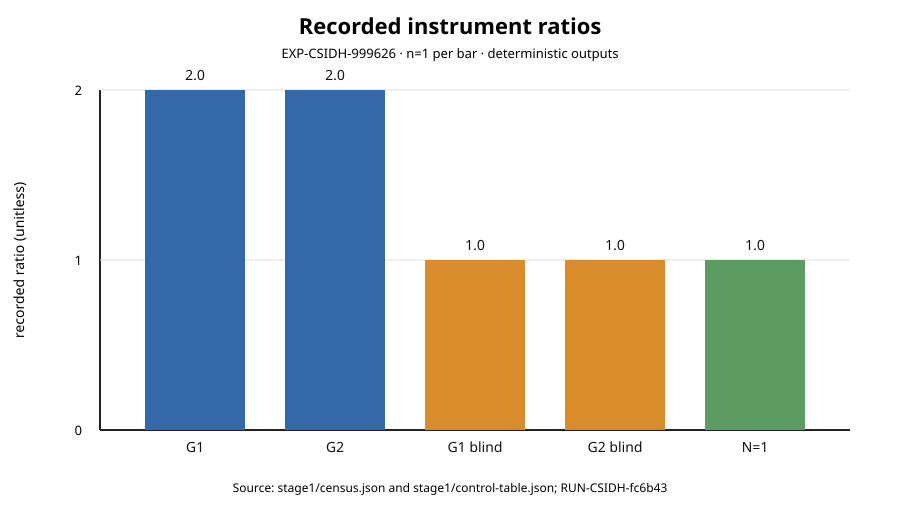
\includegraphics[width=0.98\linewidth]{graph.svg}
\caption{Recorded deterministic ratios ($n=1$ per bar) from \texttt{RUN-CSIDH-8a996d} and \texttt{RUN-CSIDH-fc6b43}. Values are copied from the stage artifacts; no new samples or uncertainty estimate was added.}
\end{figure}

The main ratios were 2.0 at both G levels; the blind ratios and forced-$N=1$ control were 1.0. No spread, CPU-time measurement, per-stage wall-time measurement, random seed, or statistical uncertainty was recorded, so those fields remain missing.

\section*{Artifact pointers}
The exact receipts, raw results, manifests, checker logs, and stage artifacts are in the two run directories named above. The editable graph data are in \texttt{graph-data.json}; the narrative and exact outer command are in \texttt{report.md}. This report does not generalize the deterministic ratios beyond the frozen tested scope.
\end{document}
